%\documentclass[aps,prl,reprint]{revtex4-2}
\documentclass[aps,prl,superscriptaddress,twocolumn]{revtex4}
%\documentclass[aps,prl,twocolumn]{revtex4-2}
%\documentclass[pre,amsmath,amssymb,superscriptaddress,showpacs,twocolumn]{revtex4-1}
\usepackage{amsmath,amssymb,graphicx}
%\input epsf
\usepackage{amsbsy}
\usepackage{latexsym}
\usepackage{color}
\usepackage{graphicx}
\usepackage{psfrag}
\usepackage[normalem]{ulem}
\usepackage{bm}
\usepackage{url}
\usepackage{notes2bib}
%\usepackage[inline]{showlabels}
%\usepackage{float}
\usepackage{soul}

\newcommand{\red}[1]{\textcolor{red}{#1}}
\newcommand{\blue}[1]{\textcolor{blue}{#1}}
\newcommand{\be}{\begin{equation}}
\newcommand{\ee}{\end{equation}}
\newcommand{\bea}{\begin{eqnarray}}
\newcommand{\eea}{\end{eqnarray}}
\newcommand{\bq}{\mathbf{q}}
\newcommand{\bx}{\mathbf{x}}
\newcommand{\br}{\mathbf{r}}
\newcommand{\bz}{\mathbf{0}}
%\newcommand{\comment}[1]{}
\newcommand{\col}{\textcolor}
\newcommand{\comment}[1]{}


\setcounter{equation}{11}

\begin{document}

\title{\Large Supplemental Material for ``Complexity-stability relationships disordered dynamical systems''}

\author{Onofrio Mazzarisi}
\affiliation{The Abdus Salam International Centre for Theoretical Physics (ICTP), Strada Costiera 11, 34014 Trieste, Italy}
\affiliation{National Institute of Oceanography and Applied Geophysics (OGS), via Beirut 2, 34014 Trieste, Italy}

\author{Matteo Smerlak}
\affiliation{Capital Fund Management, 23 Rue de l'Université, 75007 Paris, France}


\date{\today}


\maketitle

{\it Cut-off.---} In this section we consider a case amenable to analytical treatment to exemplify the argument behind the cut-off $\Lambda$ introduced in the main text to deal with diverging moments distributions.

Consider the case of a power law distribution 
\begin{equation}
  P(x)=\frac{x^{-\beta}}{\mathcal{Z}} ,
\end{equation}
defined from 1 to $\infty$ and with 
\begin{equation}
  \mathcal{Z}=\int_1^{\infty}dxx^{-\beta}.  
\end{equation}

Let us choose $\beta=3/2$. Notice that this power law describes the behavior of the distribution we consider in the main text for our example with $\alpha=\gamma=1$ and $\beta=3/2$.
The distribution is normalized with $\mathcal{Z}=2$, but the mean diverges. However, we would like to be able to describe the behavior of the sample mean 
\begin{equation}
  \bar{x}_N\equiv\frac{1}{N}\sum_{i=1}^Nx_i,
\end{equation}

where the $x_i$ are extracted from $P(x)$.
For this purpose, we can define the quantity
\begin{equation}
  \langle x\rangle_{\Lambda}\equiv\int_1^{\Lambda}dxP(x)x,
\end{equation}
with the cut-off $\Lambda$ defined such that $\int_{\Lambda}^{\infty}dxP(x)=1/N$, i.e., such that there is statistically less than 1 variable with value above $\Lambda$ out of $N$ extracted variables. For the case $\beta=3/2$ we have 
\begin{equation}
  \frac{1}{2}\int_{\Lambda}^{\infty}dxx^{-3/2}=\Lambda^{-1/2},
\end{equation}
and therefore $\Lambda=N^2$. We have for the mean
\begin{equation}
  \langle x\rangle_{\Lambda}=\frac{1}{2}\int_1^{N^2}dxx^{-1/2} = N-1.
\end{equation}
The result is plotted in Fig.~\ref{fig: SM-cut-off}, alongside the sample mean for extractions of $N=10,$ $10^2,$ $10^3,$ $10^4,$ $10^5,$ $10^6$.

\begin{figure}[h!]
  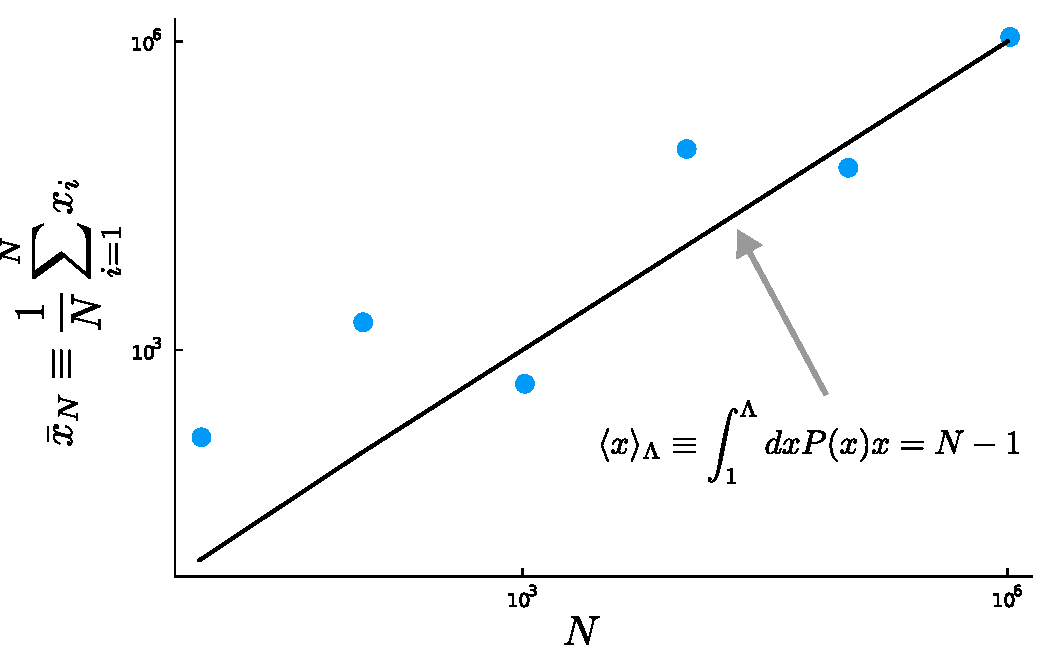
\includegraphics[width=.475\textwidth]{cut-off-justification.pdf}
  \caption{Probability of stability vs. $\sigma_e$ for a system with $S=100$, $\mu=\sigma=0.01$, $\alpha=\gamma=1$ and $\beta=3/2$.
  }
  \label{fig: SM-cut-off}
\end{figure}

{\it Heterogeneous exponents.---} In this section we explore the robustness of our findings in the case in which the exponents characterizing the dynamics of each degree of freedom $x_i$ are not identical for all $i$.

Consider the system
\begin{equation}
  \dot{x}_i = x_i^{\alpha_i} - \sum_jA_{ij}x_i^{\beta_i}x_j^{\gamma_i}
\end{equation}
where the exponents $\alpha_i$, $\beta_i$, $\gamma_i$, are extracted from Gaussian distributions: $\alpha_i\sim\mathcal N(\alpha,\sigma_e)$, $\beta_i\sim\mathcal N(\beta,\sigma_e)$ and $\gamma_i\sim\mathcal N(\gamma,\sigma_e)$, respectively with mean $\alpha$, $\beta$ and $\gamma$, and with the same standard deviation $\sigma_e$. The interaction coefficients $A_{ij}$ are drawn independently from a distribution with mean $\mu$ and standard deviation $\sigma$.
Our results are robust when $\sigma_e$ is small enough and we observe a loss of stability when $\min_i\beta_i>\max_i\alpha_i$.
As an example, we show in the plot in Fig.~\ref{fig: SM-het-exp} the probability of stability vs. $\sigma_e$ for a system with $S=100$, $\mu=\sigma=0.01$, $\alpha=\gamma=1$ and $\beta=3/2$.
The probability of stability is obtained as the fraction of stable systems out of $100$ realizations for each value of $\sigma_e$.

\begin{figure}[h!]
  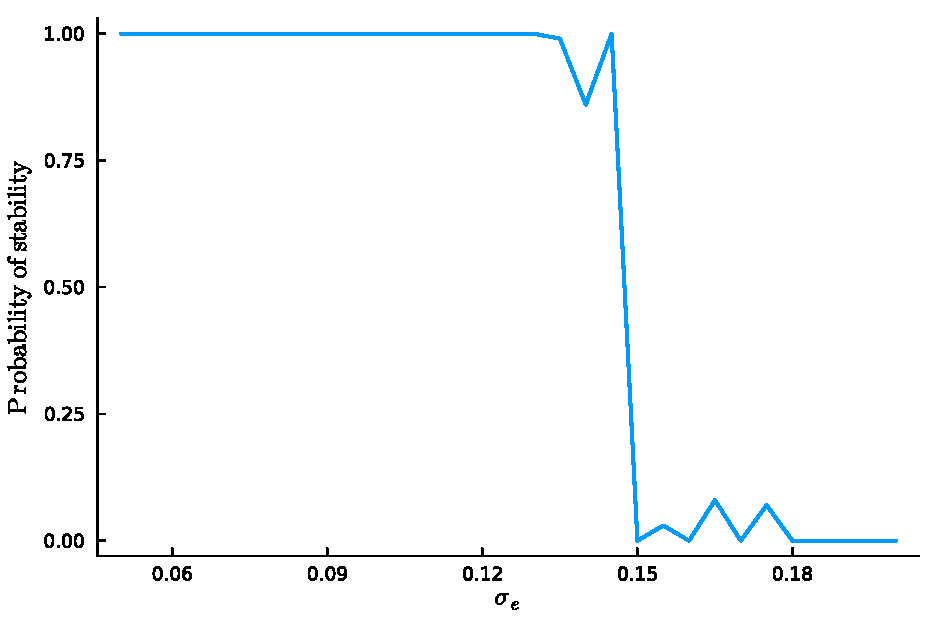
\includegraphics[width=.475\textwidth]{stoch-exp.pdf}
  \caption{Probability of stability vs. $\sigma_e$ for a system with $S=100$, $\mu=\sigma=0.01$, $\alpha=\gamma=1$ and $\beta=3/2$.
  }
  \label{fig: SM-het-exp}
\end{figure}

\end{document}
